\documentclass[12pt,a4paper]{article}

\usepackage{fontspec}
\setmainfont{Times New Roman}
\setmonofont{Menlo}[Scale=0.82]
\usepackage[brazil]{babel}
\usepackage[a4paper,left=3cm,right=2cm,top=2.5cm,bottom=2cm]{geometry}
\usepackage{setspace}
\usepackage{graphicx}
\usepackage{float}
\usepackage{booktabs}
\usepackage{array}
\usepackage{caption}
\usepackage{titlesec}
\usepackage[hidelinks]{hyperref}

\titleformat{\section}{\normalfont\bfseries}{}{0pt}{}
\titlespacing*{\section}{0pt}{1.1\baselineskip}{0.4\baselineskip}
\captionsetup{labelsep=endash,font=small,justification=centering}
\newcommand{\code}[1]{\texttt{\detokenize{#1}}}
\setlength{\fboxsep}{1pt}
\setlength{\emergencystretch}{3em}
\setlength{\parindent}{1.25cm}

\begin{document}
\onehalfspacing

% ---- Cabecalho ----
\begin{center}
{\footnotesize
PONTIFÍCIA UNIVERSIDADE CATÓLICA DO RIO GRANDE DO SUL — LABORATÓRIO DE REDES DE COMPUTADORES\par}
\vspace{0.4cm}
{\bfseries\large INTERCEPTAÇÃO E DEFESA DE UM PROTOCOLO DE APLICAÇÃO\par}
{\bfseries Fase 1: reconhecimento e escuta passiva\par}
\vspace{0.2cm}
{\footnotesize Bernardo Garcia \quad Gabriel Vieira \quad Guilherme Cavazzotto \quad — \quad Porto Alegre, 2026\par}
\end{center}
\vspace{0.3cm}

\section{Objetivo}

Demonstrar na prática por que um protocolo de aplicação sem proteção quebra a
confidencialidade. Para isso construímos um serviço alvo que se comunica em
texto claro e um interceptador passivo que lê esse tráfego direto da rede, sem
participar da comunicação.

\section{Serviço alvo: protocolo KVP}

O serviço alvo é o KVP (\emph{Key-Value Protocol}), um repositório chave-valor
com login. É orientado a linha, usa UTF-8 e roda sobre TCP na porta 5050, sem
cifragem e sem \emph{hash} de senha, portanto tudo trafega legível. As
credenciais vão no comando \code{LOGIN} e os dados nos comandos \code{SET} e
\code{GET}. As credenciais de teste são o usuário \code{admin} com a senha
\code{s3nh4-pucrs}.

\begin{table}[H]
\centering
\small
\begin{tabular}{@{}>{\raggedright\arraybackslash}p{4.8cm} >{\raggedright\arraybackslash}p{8.7cm}@{}}
\toprule
\textbf{Comando} & \textbf{Efeito} \\
\midrule
\code{LOGIN <usuario> <senha>} & Autentica a sessão (credenciais em texto claro). \\
\code{SET <chave> <valor>} & Grava um valor. \\
\code{GET <chave>} & Lê um valor. \\
\code{DEL <chave>} & Remove um valor. \\
\code{LIST} & Lista as chaves. \\
\code{PING} / \code{QUIT} & Testa a conexão / encerra a sessão. \\
\bottomrule
\end{tabular}
\end{table}

\section{Interceptador passivo (sniffer)}

O sniffer usa um socket \emph{raw} (\code{AF_PACKET}, \code{SOCK_RAW}), sem
biblioteca de captura pronta. Ele recebe os quadros Ethernet da interface, faz o
\emph{parsing} manual de Ethernet, IPv4 e TCP, filtra a porta 5050 e imprime o
conteúdo da aplicação, destacando as linhas sensíveis (\code{LOGIN}, \code{SET},
\code{GET}, \code{VALUE}). Ele apenas escuta, não envia nada: um observador
totalmente passivo já lê tudo o que passa.

\section{Ambiente de teste}

O teste foi feito em um único host, com duas captações independentes do mesmo
tráfego: o Wireshark (via \code{tshark}) na interface \code{lo0} do macOS, e o
sniffer próprio em um Linux (contêiner, kernel 6.12) na interface \code{lo},
pois \code{AF_PACKET} só existe no Linux. O conteúdo é idêntico ao do cenário de
três VMs (VM-cliente, VM-servidor e VM-observador) descrito no \code{README.md}.
O cliente roda em modo demonstração e envia, em sequência: \code{PING},
\code{LOGIN admin s3nh4-pucrs}, \code{SET cartao 4111-1111-1111-1111},
\code{SET cofre senha-do-cofre-123}, \code{GET cartao}, \code{LIST} e
\code{QUIT}.

\section{Evidências de captura}

A Figura~\ref{fig:sniffer} mostra parte da saída do sniffer próprio. A senha do
\code{LOGIN}, o número de cartão e a senha do cofre aparecem legíveis, lidos por
um processo que nunca conversou com o servidor. Cada \emph{payload} aparece duas
vezes (por exemplo, os pacotes 7 e 8 com o mesmo \code{LOGIN}): é o
comportamento do \emph{loopback} no Linux, onde o \code{AF_PACKET} vê o pacote na
saída e na entrada da interface \code{lo}; em um segmento Ethernet real cada
pacote apareceria uma vez.

\begin{figure}[H]
\centering
\caption{Saída do sniffer próprio com o conteúdo em texto claro.}
\label{fig:sniffer}
\fbox{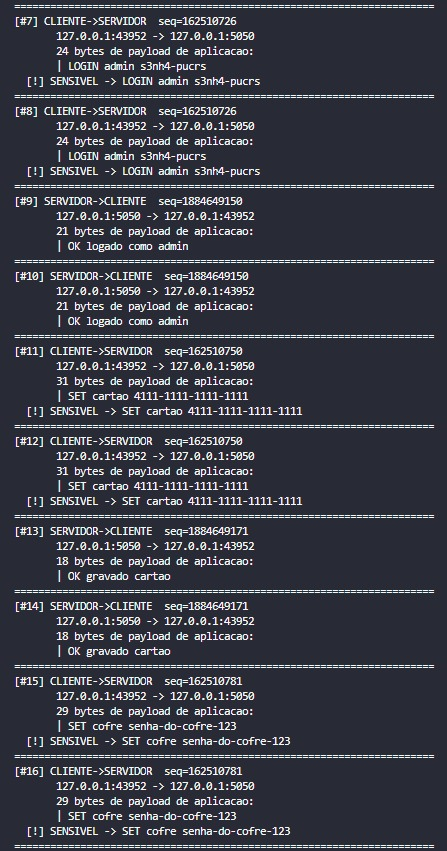
\includegraphics[width=0.5\linewidth]{capturas/fig1-sniffer.jpg}}
\end{figure}

As Figuras~\ref{fig:login} e~\ref{fig:stream} mostram o mesmo tráfego no
Wireshark. Na primeira, o pacote 19 está selecionado e o painel de bytes exibe
\code{LOGIN admin s3nh4-pucrs} em ASCII. Na segunda, a função \emph{Follow TCP
Stream} remonta a conexão inteira, com o cliente em vermelho e o servidor em
azul.

\begin{figure}[H]
\centering
\caption{Pacote 19 com o comando LOGIN em texto claro (Wireshark).}
\label{fig:login}
\fbox{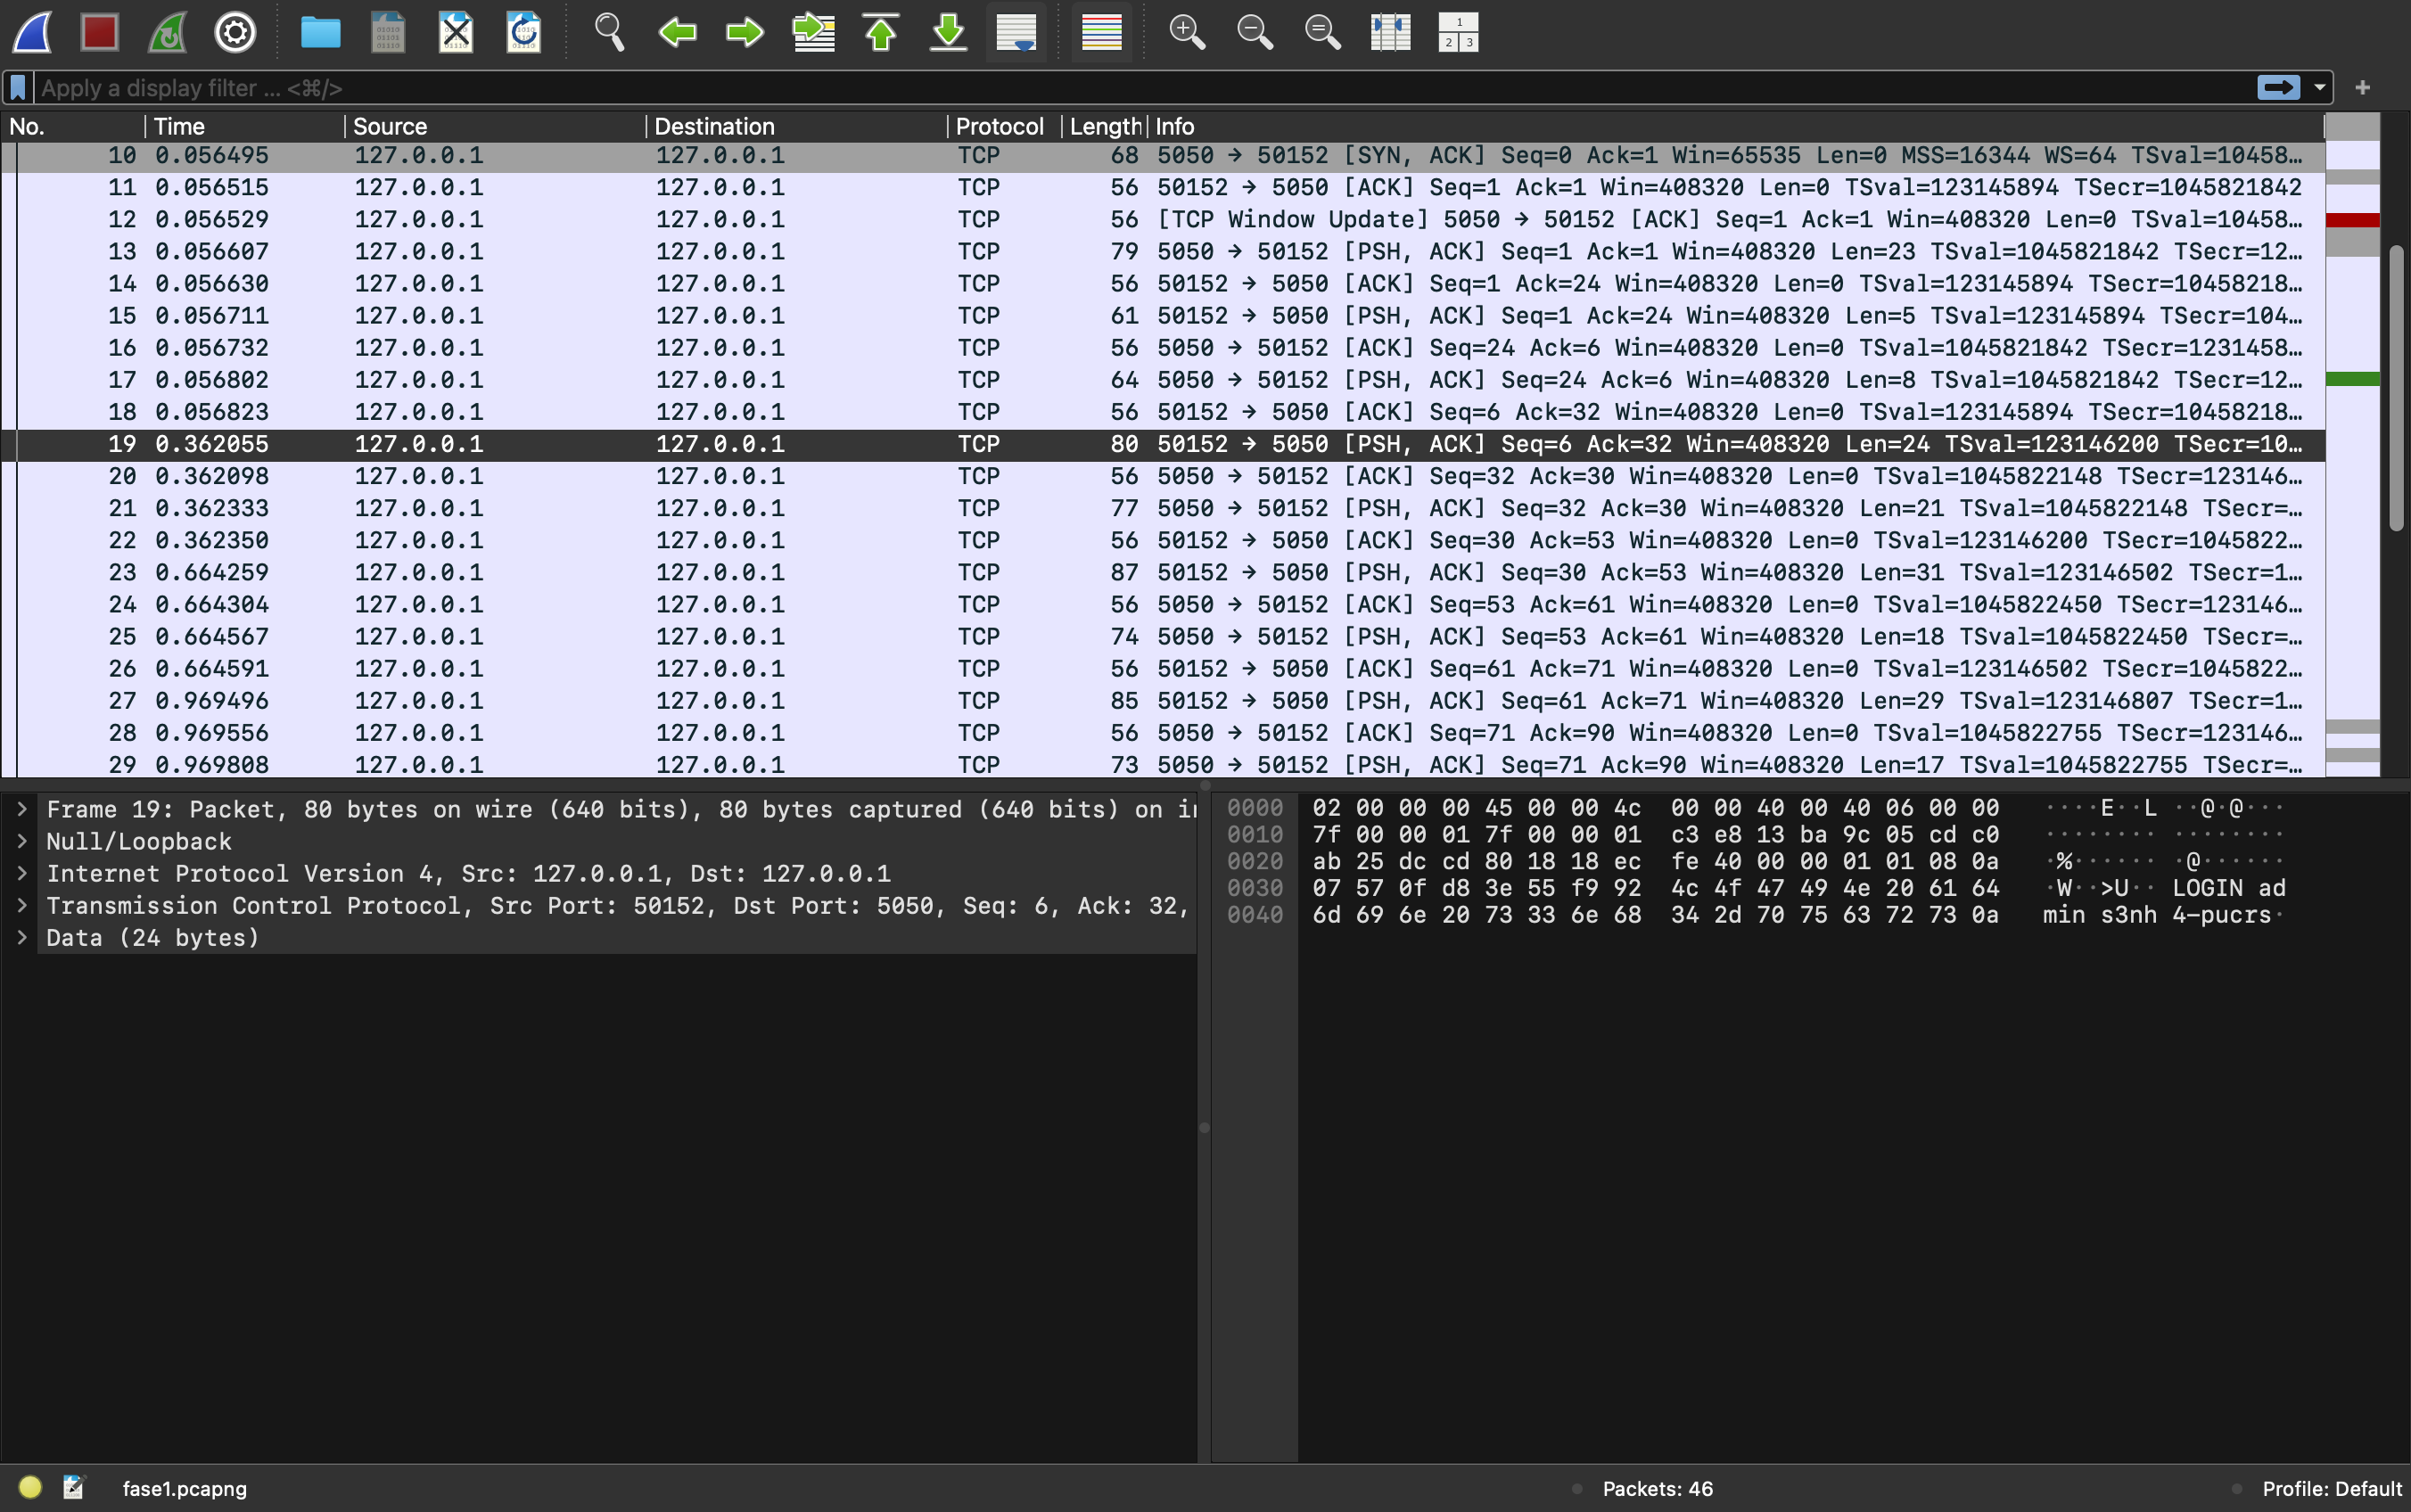
\includegraphics[width=0.98\linewidth]{capturas/fig2-wireshark-login.png}}
\end{figure}

\begin{figure}[H]
\centering
\caption{Conversa completa reconstruída (Follow TCP Stream).}
\label{fig:stream}
\fbox{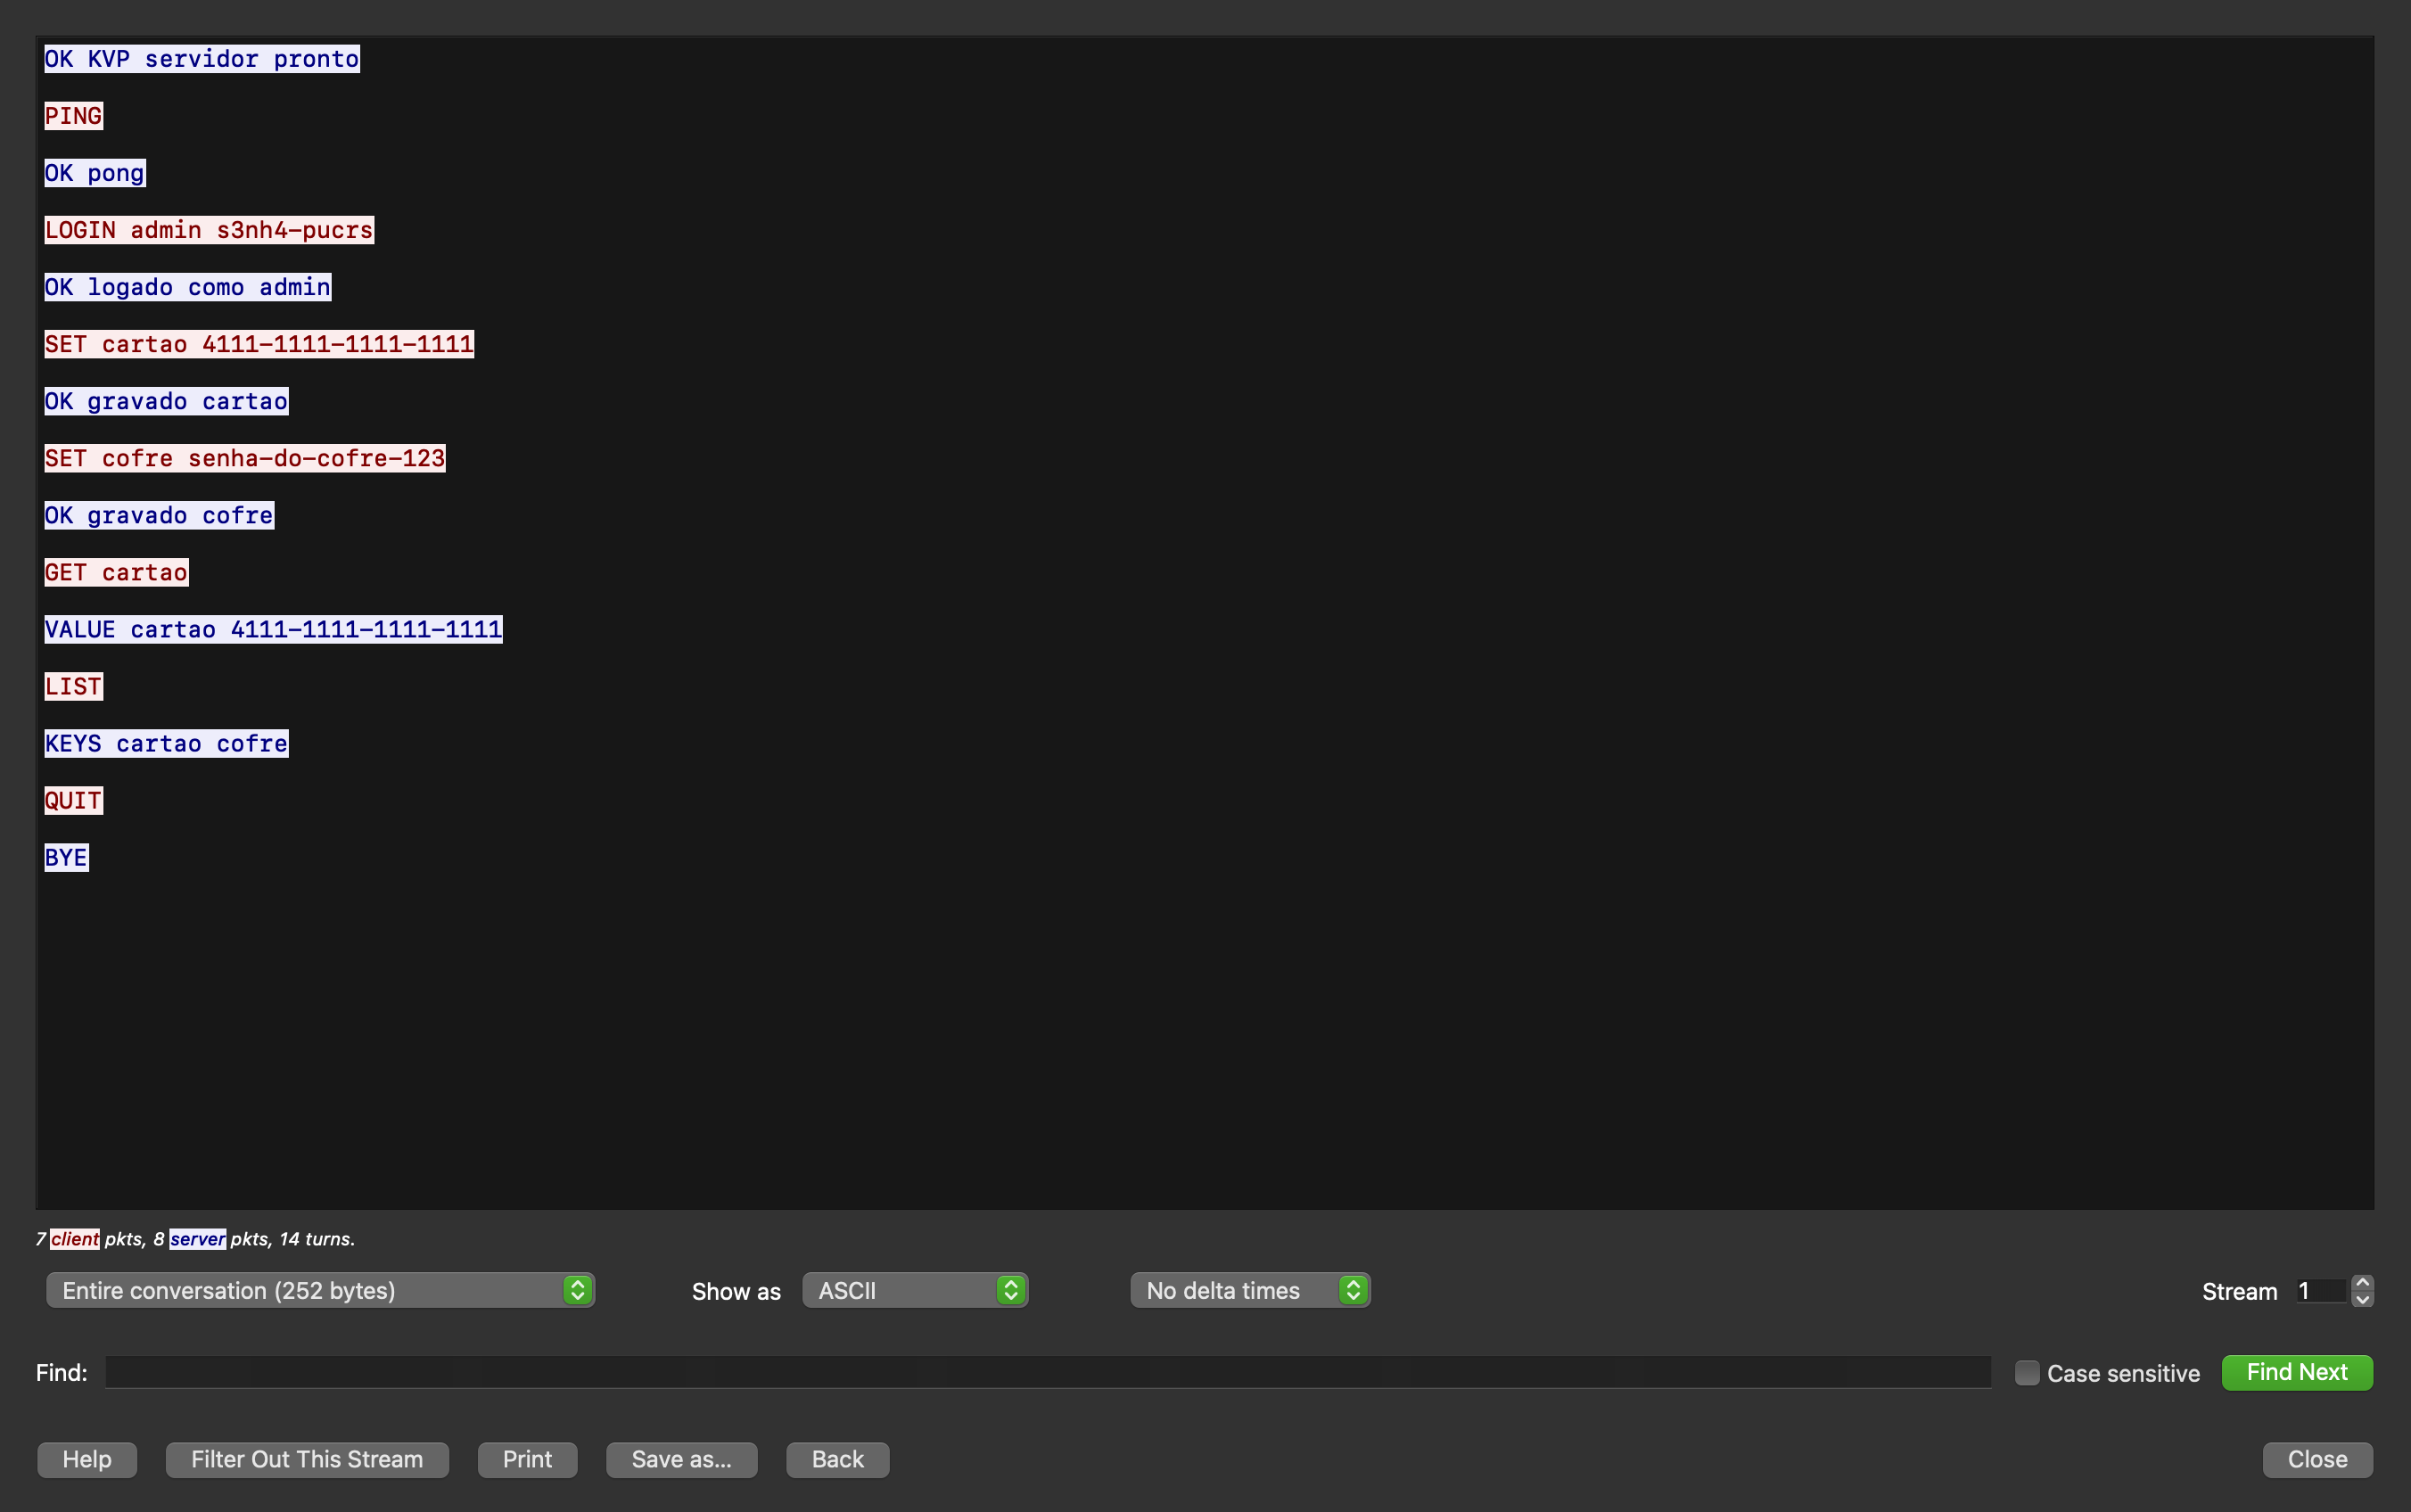
\includegraphics[width=0.98\linewidth]{capturas/fig3-wireshark-stream.png}}
\end{figure}

A Tabela~\ref{tab:pacotes} lista os pacotes com conteúdo de aplicação da conexão
\code{127.0.0.1:50152 -> 127.0.0.1:5050}, com o número de cada pacote e o texto
observado. As linhas em negrito são as de dado sensível.

\begin{table}[H]
\centering
\caption{Pacotes com conteúdo legível na captura do Wireshark.}
\label{tab:pacotes}
\footnotesize
\begin{tabular}{@{}c l >{\raggedright\arraybackslash}p{6.6cm}@{}}
\toprule
\textbf{Pacote} & \textbf{Sentido} & \textbf{Conteúdo observado} \\
\midrule
\textbf{19} & cliente $\rightarrow$ servidor & \textbf{\code{LOGIN admin s3nh4-pucrs}} \\
21 & servidor $\rightarrow$ cliente & \code{OK logado como admin} \\
\textbf{23} & cliente $\rightarrow$ servidor & \textbf{\code{SET cartao 4111-1111-1111-1111}} \\
\textbf{27} & cliente $\rightarrow$ servidor & \textbf{\code{SET cofre senha-do-cofre-123}} \\
31 & cliente $\rightarrow$ servidor & \code{GET cartao} \\
\textbf{33} & servidor $\rightarrow$ cliente & \textbf{\code{VALUE cartao 4111-1111-1111-1111}} \\
37 & servidor $\rightarrow$ cliente & \code{KEYS cartao cofre} \\
\bottomrule
\end{tabular}
\end{table}

\section{Conclusão}

As duas ferramentas leem as credenciais e os valores em texto claro, sem nenhum
esforço de decodificação. A causa é a ausência de cifragem no canal (sem TLS):
qualquer byte enviado vira texto visível, e o atacante passivo não precisa
autenticar nem enviar nada. Na Fase 3, o canal receberá TLS e as senhas passarão
a usar \emph{hash}; com isso, o sniffer desta fase deixará de conseguir ler o
conteúdo.

\end{document}
